\section{Systementwurf}

\label{sec_impl_architecture}

In diesem Abschnitt wird basierend auf den Anforderungen aus Abschnitt \ref{sec_impl_requirements} eine von den eingesetzten Verfahren unabhängige Architektur für das System entworfen. Der erste Abschnitt beschäftigt sich mit der Frage, an welcher Stelle in den Datenfluss zwischen Quelle der Logdaten und SIEM-System eingriffen werden kann. Im anschließenden Abschnitt wird hierauf basierend die Systemarchitektur erstellt.

\subsection{Eingriff in den Datenfluss des SIEM-Systems}

\label{sec_over_dataflow_siem}

\todo{EZ: Hier interessieren insbesondere auch die Auswirkungen auf den Rest des Systems? Wie muss das Schwellwertschema angepasst werden? Welche Akteure wissen zu welchem Zeitpunkt was? Wer bekommt welche Schluessel? Usw... Der Abschnitt hat also wesentlich mehr Potential!}

Für den Eingriff zur Pseudonymisierung der Logdaten bieten sich verschiedene Stellen im Datenfluss eines SIEM-Systems an. Im Folgenden werden diese Möglichkeiten dargestellt und bezogen auf die jeweils resultierenden Eigenschaften einer Möglichkeit bewertet:

\begin{itemize}

  \item \textbf{Veränderung des SIEM-Systems: } Muss das eingesetzte SIEM-System für die Umsetzung der Lösung angepasst werden? Dies wäre im Hinblick auf zukünftige Updates, die das SIEM-System durch seinen Entwickler erfährt, nicht wünschenswert, da jedes dieser Updates dafür sorgen könnte, dass die umgesetzte Lösung angepasst werden muss. Weiterhin würde dieser Ansatz ein SIEM-System erfordern, das entweder quelloffen vorliegt und verändert werden darf oder das die gewünschte Verhaltensänderung zumindest durch Erweiterungen zulässt. 
  
  \item \textbf{Nicht-pseudonymisierte Daten im SIEM-System: } Um das Ziel der Arbeit -- die Pseudonymisierung, die nur durch Kollaboration aufgedeckt werden kann -- zu erreichen, muss sichergestellt sein, dass Logdaten nirgendwo in nicht-pseudonymisierter Form vorliegen. Da insbesondere das zukünftige Verhalten des SIEM-Systems nicht beeinflusst werden kann, wäre es wünschenswert, dass die Logdaten das SIEM-System bereits in pseudonymisierter Form erreichen.\\
  Die Relevanz dieser Eigenschaft lässt sich am Beispiel des später in dieser Arbeit genutzten SIEM-Systems OSSIM erkennen: Wird das Syslog-Protokoll genutzt, um Logdaten in OSSIM aufzunehmen, so werden die Einträge erst in einer Logdatei abgelegt und von dort aus geparst, normalisiert und in der Datenbank gespeichert. Das Datum verbleibt in der Logdatei. Kommen die Daten in nicht-pseudonymisierter Form in dem OSSIM-Sensor an, so muss sichergestellt werden, dass verarbeitete Einträge gelöscht oder verändert werden.
  
  \item \textbf{Mehrfaches Parsen von Logdaten: } Durch das SIEM-System werden die Logdaten - wie in Abschnitt \ref{sec_basics_siem} beschrieben - geparst und normalisiert. Aus Performancegründen ist eine Lösung zu bevorzugen, die diesen Vorgang oder Teile davon nicht mehrfach voraussetzt.
  
  \item \textbf{Abhängigkeit von Besonderheiten des SIEM-Systems: } Einige SIEM-Systeme bieten die Möglichkeit der verteilten Installation oder andere spezifische Eigenschaften. Eine Lösung, die unabhängig von dem verwendeten SIEM-System funktioniert, ist zu bevorzugen, da sie universell einsetzbar ist.    
  
%  \item \textbf{Manipulierbarkeit auf den Übertragungswegen(?): }

\end{itemize}


Eine Übersicht über die verschiedenen Stellen des Eingriffs bietet Abbildung \ref{fig:siem_data_access_point}. Die dort mit Ziffern gekennzeichneten Möglichkeiten sind:

\begin{figure}[]
    \centering
        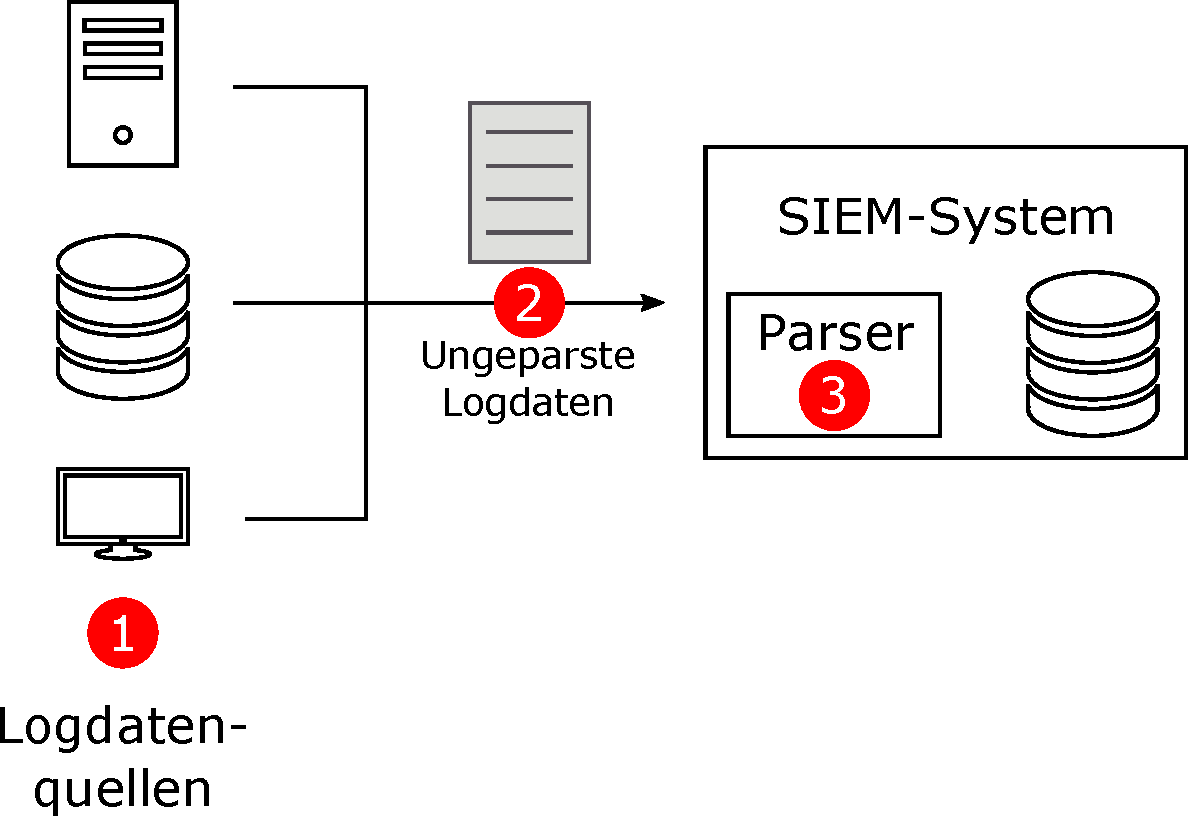
\includegraphics[width=0.5\textwidth]{dia/siem_data_access_point.pdf}
    \caption{Mögliche Eingriffspunkte in den Datenfluss eines SIEM-Systems.}
    \label{fig:siem_data_access_point}
\end{figure}

\begin{enumerate}

\item \textbf{In der Quelle der Logdaten}\\
  Bei diesem Ansatz werden die Daten bereits verädert, bevor sie die Datenquelle verlassen. Dieser Ansatz sorgt dafür, dass die Daten bereits pseudonymisiert auf der Übertragungsstrecke und im SIEM-System vorliegen. Es ist kein mehrfaches Parsen der Daten notwendig und der Ansatz ist unabhängig vom verwendeten SIEM-System zu realisieren. Auf der anderen Seite macht der Ansatz die Veränderung generell jeder Datenquelle notwendig. Dies kann bei Datenquellen, die auf ähnlichen gut erweiterbaren Plattformen beruhen, relativ einfach umzusetzen sein. Beispielsweise könnte die im nächsten Ansatz vorgestellte Proxy-Komponente lokal auf der Datenquelle eingesetzt werden. Schwierigkeiten würde dieser Ansatz hingegen bei Datenquellen bereiten, die beispielsweise aus Gründen abgespeckter zugrundeliegender Betriebssysteme oder wegen geringer Rechenleistung nur schwer erweiterbar sind. Außerdem würde der Ansatz in vielen Fällen die Kooperation des Herstellers voraussetzen, wenn es sich um nicht quelloffene \glqq{}Box\grqq{}-Lösungen handelt.

\item \textbf{Proxy-basierter Ansatz}\\
  Dieser Ansatz pseudonymisiert die Daten vor dem ersten Kontakt mit dem SIEM-System, indem Datenquellen ihre Logdaten an einen Proxy senden, der die Daten pseudonymisiert und erst anschließend an das SIEM-System weiterreicht. Hierdurch wird erreicht, dass die Daten zu keiner Zeit nicht-pseudonymisiert im SIEM-System vorliegen. Der Ansatz ist unabhängig von den Datenquellen und dem SIEM-System und erfordert somit keinen direkte Eingriffe (abgesehen von geringen Konfigurationsanpassungen). Ein Nachteil dieser Lösung ist, dass sie das Parsen und Neuzusammensetzen der Logdaten im Proxy zusätzlich zu deren anschließender Behandlung im SIEM-System erfordert. Außerdem müssen für verschiedene Arten der Logdatenübermittlung (Protokolle wie Syslog oder SNMP) unterschiedliche Proxys entwickelt werden.

\item \textbf{Patchen des SIEM-Systems}\\
  Die dritte Möglichkeit ist das Verändern des SIEM-Systems selbst. Hierzu wird in die Logdaten parsende Komponente eingegriffen, um vor, während oder nach diesem Vorgang die Logdaten zu pseudonymisieren. Dieser Ansatz erfordert kein mehrfaches Bearbeiten von Logdaten wie im proxybasierten Ansatz. Auf der anderen Seite ist er abhängig vom eingesetzten SIEM-System und erfordert seine Veränderung. Zusätzlich liegen die Daten erst einmal in nicht veränderter Form im SIEM-System vor, was die in Abschnitt \ref{subsec_impl_requirements_ossimintegration} erwähnten Nachteile mit sich bringt.

\end{enumerate}

Aus datenschutztechnischer Sicht ist eine frühestmögliche Pseudonymisierung zu bevorzugen, wie sie auch in \cite{schwartmann2017} empfohlen wird: 
\glqq{}Die Pseudonymisierung ist im Verarbeitungsprozess so früh wie möglich durchzuführen.\grqq{}
Daher wäre eine Pseudonymisierung bereits in der Datenquelle der Optimalfall. Demgegenüber stehen jedoch die erwähnten Umsetzbarkeits-Nachteile des ersten Ansatzes, da hierzu jede mögliche Quelle von Logdaten verändert werden müsste. Eine erst im SIEM-System stattfindende Pseudonymisierung bringt jedoch die beschriebenen Risiken des Vorliegens pseudonymisierter Daten im Originalformat mit sich.

Dies begründet die Entscheidung für den proxybasierten Ansatz. Dass die Lösung außerdem noch keine Anpassungen an dem SIEM-System selbst erfordert, wiegt den Nachteil des zusätzlichen Parsens und Wiederzusammensetzens der Lognachricht bei Weitem auf.
\todo{Auch auf Angreifermodell beziehen?}

\subsection{Architektur}

\label{sec_over_architecture}

%- Wie deckt dieser Ansatz die Anforderungen ab?
%  - Einbindung OSSIM
%  - Pseudonymisierung
%  - Schwellwert
%  - Benutzerinteraktion
%  - Erweiterbarkeit Datenquellen
%  - Erweiterbarkeit Datenschutztechniken

Ausgehend von diesen Überlegungen wird ein System entworfen, das die Anforderungen aus Abschnitt \ref{sec_impl_requirements} erfüllt und proxybasiert in den Datenfluss eingreift. 

%\todo{Hier erweitern: Warum verteilte Lsg (ProxyPlugin - Service):
%  - Erweiterbarkeit (Mehrere Proxy-Server mit verschiedenen Protokollen, evtl. auch direkt Client-seitig, ...) => Absicherung einer Komponente, die jedoch auch nicht alles erfährt
%  - Trennung Verarbeitung und Speicherung (Kompr. DB -> Pseudonyme bleiben verdeckt, Kompr. Proxy -> bisherige Daten und Daten evtl. anderer Proxys bleiben abgesichert)
%}

Bei dem Entwurf handelt es sich um ein verteiltes System, bei dem die Verarbeitung der Logdaten und die Speicherung der Pseudonymzuordnung an unterschiedlichen Stellen geschieht. Hierfür sprechen verschiedene Gründe. Die Kompromittierung der speichernden Komponente schützt die erstellten Pseudonyme vor Aufdeckung durch die Verschlüsselung der Datensätze mit einem kryptographischen Schwellwertschema. Die Kompromittierung der verarbeitenden Komponente lässt zwar eine Verknüpfung neu erstellter Pseudonyme mit eintreffenden Daten zu, sorgt aber nicht für eine Aufdeckung bereits erstellter Pseudonyme, da diese in der anderen Komponente vorliegen.

Weiterhin sorgt dieser Ansatz auch für eine zusätzliche Erweiterbarkeit des Systems. Eine speichernde Komponente kann so als Datenspeicher für mehrere verarbeitende Komponenten agieren, was beispielsweise die Erweiterung um zusätzliche Protokolle (vgl. Abschnitt \ref{sec_impl_integration_into_ossim}) oder Pseudonyme über verschiedene Datenarten (vgl. Abschnitt \ref{sec_state_se_furtherpossibilities}) ermöglicht.

Einen Überblick über den Entwurf bietet Abbildung \ref{fig:high__level_architecture}. Die verschiedenen Komponenten des Systems werden im Folgenden näher beschrieben.

\begin{figure}[]
    \centering
        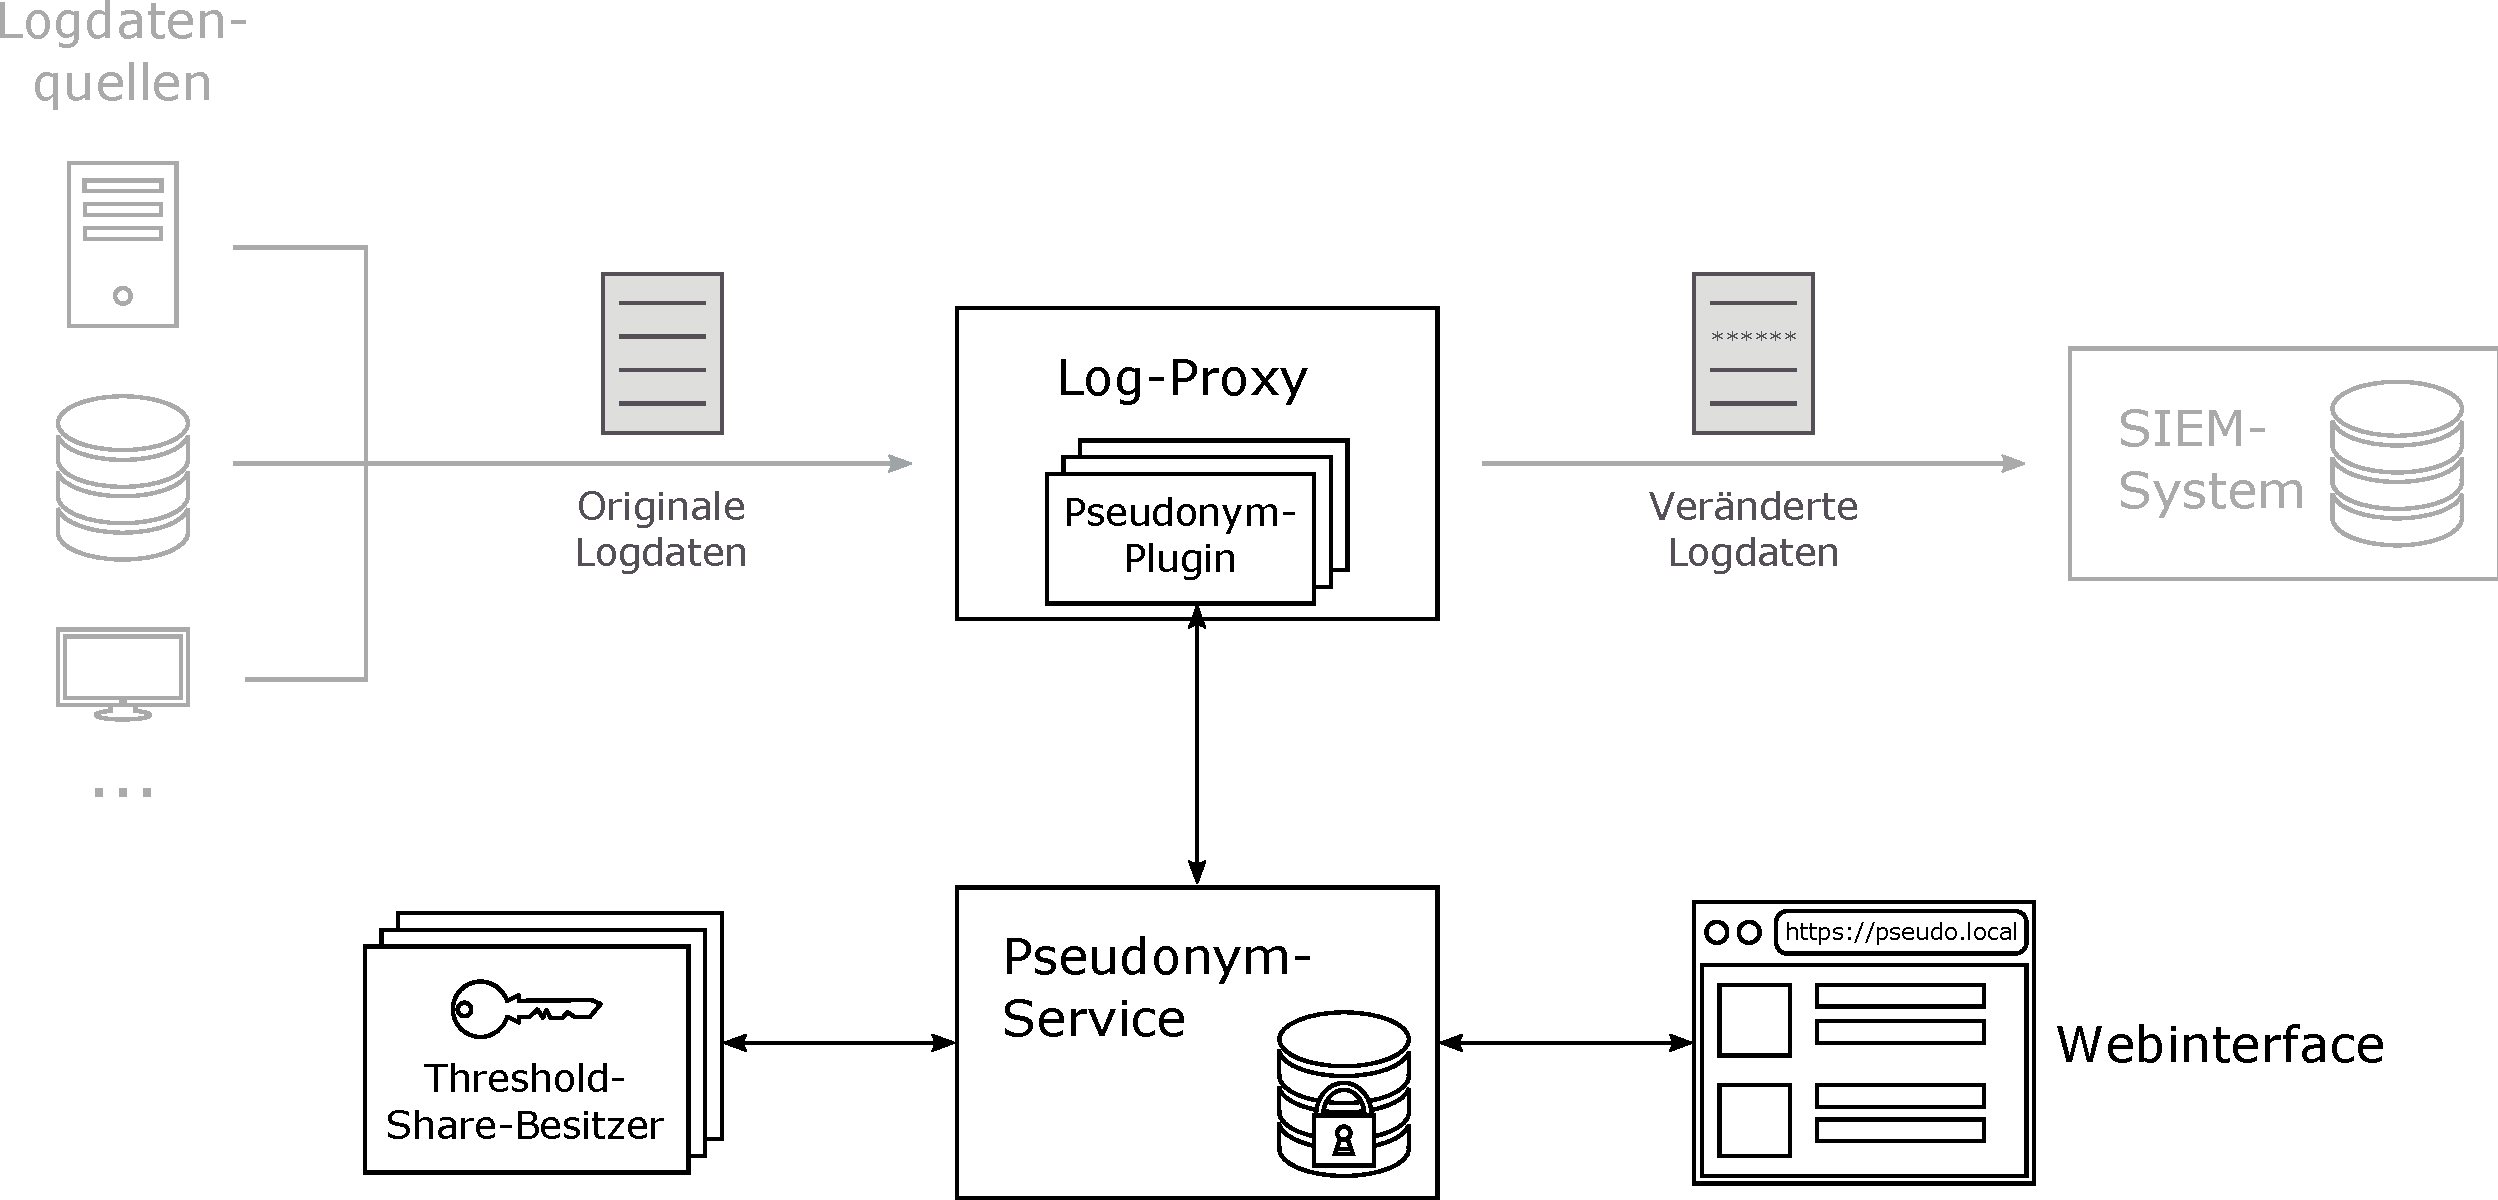
\includegraphics[width=0.9\textwidth]{dia/high_level_architecture.pdf}
    \caption{Ein Überblick über die entworfene Architektur.}
    \label{fig:high__level_architecture}
\end{figure}

Die erste Komponente ist der \textbf{Log-Proxy}, der die Daten entgegennimmt, verändert und anschließend an das SIEM-System weiterleitet. Das Verändern der Daten kann mit verschiedenen Plugins geschehen, so dass neben der umzusetzenden Pseudonymisierung auch weitere Datenschutztechniken eingesetzt werden können, was die geforderte Erweiterbarkeit aus Abschnitt \ref{subsec_impl_requirements_plugins} ermöglicht. Der Proxy leistet die Behandlung von Logdaten aus verschiedenen Quellen wie in Abschnitt \ref{subsec_impl_requirements_differentsources} beschrieben. Das für diese Art des Dateneingriffs erforderliche Parsen und Wiederzusammensetzen der Daten muss hier datenquellenabhängig zu konfigurieren sein.

Ein in dem Proxy enhaltenes Plugin ist für die Pseudonymisierung von Daten zuständig und kommuniziert dazu mit einer externen Komponente -- dem Pseudonym-Service. Die Kommunikation mit dem Proxy erfolgt über einen webservicebasierten Ansatz. Das Plugin kann für eingehende Daten ein Pseudonym anfordern und dieses anschließend in der Logdatenverarbeitung verwenden.

Der \textbf{Pseudonym-Service} erfüllt zwei Aufgaben: Speichern und Verwalten der Pseudonyme sowie die Integration des kryptographischen Schwellwertschemas. Initial muss die Schlüsselgenerierung des Schwellwertschemas durch den Service geleistet werden. Dies kann wie bereits im vorhergehenden Abschnitt beschrieben zentral oder verteilt geschehen.

Während des Betriebs können  neue Pseudonyme angelegt und zusammen mit ihrem durch das Schwellwertschema verschlüsselten Datum abgelegt werden. Sie werden durch geeignete Maßnahmen durchsuchbar gehalten, um für ein Datum überprüfen zu können, ob bereits ein Pseudonym vergeben wurde (dieses Problem wird in Abschnitt \ref{sec_state_se} genauer dargestellt).\\
Über ein Webinterface kann ein berechtiger Benutzer die Aufdeckung eines bestimmten Pseudonyms fordern und den Status seiner Forderung bzw. im Erfolgsfall das aufgedeckte Datum betrachten. Dieses Datum wird durch das Kombinieren der partiellen Entschlüsselungen erhalten, die von den entsprechenden \textit{Share}-Besitzern berechnet werden. Weiterhin kann über dieses Webinterface auch die initiale Konfiguration des Systems in Bezug auf Eigenschaften der Pseudonymisierung und des kryptographischen Schwellwertschemas vorgenommen werden.

Benutzer, die über das Webinterface oder den Webservice mit dem Pseudonym-Service agieren möchten, werden durch geeignete Maßnahmen authentifiziert und ihre Autorisierung wird überprüft.

Benutzer, die für die Bewertung von Anfragen zur Aufdeckung eines Pseudonyms zuständig sind, erhalten die Möglichkeit zur Interaktion mit dem System über eine \textbf{Client-Anwendung}, für die der Pseudonym-Service ebenfalls als Webservice agiert. Diese Anwendung verwaltet den \textit{Share} des Benutzers für das kryptographische Schwellwertschema. Sie kann, nachdem der Benutzer der Aufdeckung eines Pseudonyms zugestimmt hat, die partielle Entschlüsselung eines Datensatzes berechnen und diese an den Pseudonym-Service senden.

Für alle Übertragungsstrecken wird angenommen, dass ein Angreifer keinen Zugriff auf Kommunikationsinhalte erhält oder diese verändern kann. Dies ist durch Transportverschlüsselung mittels des weitverbreiteten TLS-Protokolls zu erreichen, muss jedoch bei der Verwendung des Systems beachtet werden. 